\documentclass{jarticle}
\usepackage{robomech}
\usepackage[dvipdfmx]{graphicx}

\usepackage{amsmath} % assumes amsmath package installed
\usepackage{amssymb}  % assumes amsmath package installed

\newcommand{\argmin}{\mathop{\rm argmin}\limits}
\newcommand{\argmax}{\mathop{\rm argmax}\limits}
\newcommand{\V}[1]{\boldsymbol{#1}}

\begin{document}

\makeatletter

\title{自己位置の不確かな移動ロボットの安全な隘路通過のための引き返し行動}
{}
{A method for generating backtracking behaviors of mobile robots for safety passage in narrow paths}
{}

\author{
\begin{tabular}{c}
 ○\hspace{1zw}上田隆一 (千葉工大)\\
 {\small Ryuichi UEDA, Chiba Institute of Technology, ryuichi.ueda@p.chibakoudai.jp}
\end{tabular}
}

\makeatother

\abstract{ \small 
This paper proposes a mathematical model that makes a mobile robot retry
a motion when the robot has not enough information for doing it safely.
Outdoor mobile robots sometimes run off a road and collide with low edge stones 
even if these hazards are written in the maps for navigation due to
the uncertainty of self-localization. Our model makes a robot turn back when
a risk is expected. 
}

\date{} % 日付を出力しない
\keywords{Probabilistic Robotics, mobile robots}

\maketitle
\thispagestyle{empty}
\pagestyle{empty}

\small
\section{緒言}

レーザスキャナなどのセンサの小型化、高性能化により、
移動ロボットが屋外で自己位置推定することは容易になった。
一方で、つくばチャレンジなどで行われる走行実験では、
路肩での脱輪などで走行不能になる場面が多くみられる。
この原因としては、ロボットが自己位置推定や
ナビゲーションに利用している環境地図の不正確さや、
自己位置推定の不正確さが考えられる。

本稿では、後者の自己位置推定の不正確さに対処するための
ロボットの行動を扱う。具体的には、
ロボットがある小径を通り抜けようとするときに、
自己位置推定の正確さが足りない場合、
後戻りして再度挑戦する、という行動を発現させる
数理モデルを提案する。


\section{問題設定}\label{sec:problem}

図\ref{fig:environment}のようなシミュレーション環境を考える。
シミュレーションの詳細は\cite{上田2019}に説明されている。
ロボットのタスクは、ある位置と向きから
図中の水たまりを避けてゴールに向かうことである。
水たまりに入った場合のペナルティーとして、
時刻換算で一定のペナルティーが与えられる。

ロボットの座標は$\V{x} = (x,y,\theta)$で表される。

移動には雑音がある。

センサ情報から自己位置推定する。
推定結果は確率密度関数$b_t(\V{x})$で表される。


\begin{figure}[tbh]
 \centering
  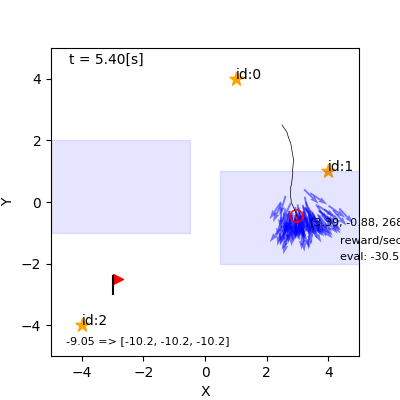
\includegraphics[width=1.0\linewidth]{figs/puddle_world.png}
  \vspace*{-4mm}
  \caption{Environment}
  \label{fig:environment}
\end{figure}

前提として、ロボットは
任意の位置と向き(合わせて以後「姿勢」と呼ぶ)
から、あるルール(方策)で行動を決定して実行した場合、
どれだけのペナルティーでゴールできるか、
期待値を知っているとする。
これは、動的計画法や強化学習における
状態価値関数に相当する。

\begin{align}
	V^\Pi: \mathcal{X} \to \Re \\
	\Pi: \mathcal{X} \to \mathcal{A}
\end{align}

\begin{align}
	r(\V{x},a,\V{x}') = - \Delta t - c d(\V{x}')
\end{align}

\section{後戻り行動}

ロボットは、後戻りをする条件になると、
$t_\text{back}$秒間だけ後戻りをすることとする。
時間$t_\text{back}$は、どれだけの時間だけ
後戻りが許容されるか、そして、
どれだけ時間をかけるとやり直しに必要な
センサ情報が得られるかを勘案して設計者が
決めることとなる。

後戻りするための方策には、
本稿では
\begin{align}
	\Pi_\text{back}(b) = \min_{a \in \mathcal{A}} \left|\langle Q(\V{x},a) \rangle_{b'(\V{x})} - \langle V(\V{x}) \rangle_{b(\V{x})} + \Delta t \right|
\end{align}
という式を用いる。
ここで、$b'$は$b$が$a$で遷移した後の信念分布である。
この方策は、遷移前後の価値の期待値の差が、
移動時間に対する負の報酬と釣り合うように
行動選択するものとなる。
つまり、一度行動すると、ゴールまでの時間の期待値が
$\Delta t$だけ増えるように行動選択するという意味となる。
単に価値が低い状態に遷移する行動を選択するものであると、
ロボットが水たまりに入って価値を下げようとするため、
このように移動時間に対する負の報酬で後戻りのための
行動選択を行う。




%\begin{table}[tb]
% \caption{Type size and typefaces for papers}
% \label{tbl: table1}
% \centering
% \footnotesize
% \begin{tabular}{|p{7zw}|l|l|l|}
%  \hline
%	適用場所	&日本語	&欧文 \\\hline
%	標準のフォント	&明朝体 9pt	&Times New Roman 9pt \\\hline
%	日本語表題	&ゴシック体 14pt	&Arial 14pt \\\hline
%	日本語副表題	&ゴシック体 12pt	&Arial 12pt \\\hline
%	英語表題	&&Times New Roman 12pt \\\hline
%	英語副表題	&&Times New Roman 10pt \\\hline
%	日本語著者名	&明朝体 10pt &\\\hline
%	英語著者名	&&Times New Roman 9pt \\\hline
%	アブストラクト・キーワード	&&Times New Roman 9pt \\\hline
%	大見出し	&ゴシック体 10pt	&Arial 10pt \\\hline
%	中見出し	&ゴシック体 9pt	&Arial 9pt \\\hline
%	図・表の番号・タイトル	 &&Times New Roman 9pt \\\hline
%	文献	&明朝体 8pt	&Times New Roman 8pt \\
%  \hline
% \end{tabular}
%\end{table}

\footnotesize
\bibliographystyle{jorsj}
\bibliography{../bibfiles/eng,../bibfiles/jpn}
%\begin{thebibliography}{99}
%
%\bibitem{Shinjuku98}
%新宿大五朗,渋谷次郎,東京 学,``キャスティングマニピュレーションに関する研究(第1報,可変長の紐状柔軟リンクを有するマニピュレータの提案とそのスイング制御法)'',機論C編, vol.64-626, pp.3854--3861, 1998.
%
%\bibitem{Shinjuku99}
%Shinjuku, D., Shibuya, J. and Tokyo, M., ``Swing Motion Control of Casting Manipulation,'' IEEE Control Systems, vol.19-4, pp.56--64, 1999.

%\end{thebibliography}

\normalsize
\end{document}
